\documentclass[12pt]{article}
\usepackage{amssymb}
\usepackage[cmex10]{amsmath}
\usepackage{verbatim}
\usepackage{courier}
\usepackage[margin=1in]{geometry}
\usepackage{setspace}
\usepackage{graphicx}
\singlespacing
\setlength{\parindent}{0pt}

\begin{document}

%%%%%%%%%%%%%%%%%%%%%%%%%%%%%%%%%%%%%%%%%%%%%%%%%%%%%%%%%%%%%%%%%%%%%%%%%%%%%%%%%%%%%%

\section*{Imaginary Numbers}
An imaginary number $a+jb$, has magnitude $M = \sqrt{a^2+b^2}$, and phase $\phi = \tan^{-1}(b/a)$\\

\begin{center}
	$a+jb = Me^{-j\phi} = M\angle\phi $
\end{center}
Where $j = i = \sqrt{-1}$

%%%%%%%%%%%%%%%%%%%%%%%%%%%%%%%%%%%%%%%%%%%%%%%%%%%%%%%%%%%%%%%%%%%%%%%%%%%%%%%%%%%%%%

\section*{KVL/KCL}
KVL $\rightarrow$ The sum of all voltages in a loop must be zero. \\
KCL $\rightarrow$ The sum of currents in and out of a node must be zero. \\

\begin{center}
	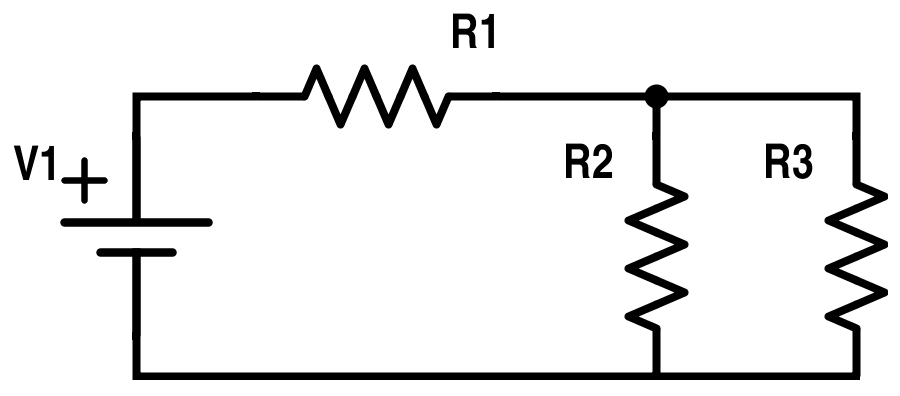
\includegraphics[width=0.8\textwidth]{assets/ece210-kvl.png}
\end{center}

KVL example, using ``positive'' as $+\rightarrow-$:
\begin{center}
	$-V_1 + V_{R1} + V_{R2} = 0$\\
	$-V_1 + V_{R1} + V_{R3} = 0$\\
	$-V_{R2} + V_{R3} = 0$
\end{center}

KCL example, using the node where the resistors meet:
\begin{center}
	$i_{R1} = i_{R2} = i_{R3}$
\end{center}


%%%%%%%%%%%%%%%%%%%%%%%%%%%%%%%%%%%%%%%%%%%%%%%%%%%%%%%%%%%%%%%%%%%%%%%%%%%%%%%%%%%%%%

\section*{Impedance}
Resistors have real resistance $R = V/I$, measured in Ohms ($\Omega$)\\
Resistors in series add cumulatively: $R_{ser} = R_1+R_2$\\
Resistors in parallel add inversely:  $1/R_{par} = 1/R_1 + 1/R_2$, or $R_{par} = \dfrac{R_1R_2}{R_1+R_2}$\\

\newpage

Capacitors have imaginary reactance $I = C \dfrac{\partial V}{\partial t}$, or $Z_c = 1/j\omega C$, measure in Farads (F)\\
Capacitors in series add inversely: $1/C_{ser} = 1/C_1 + 1/C_2$, or $C_{ser} = \dfrac{C_1C_2}{C_1+C_2}$\\
Capacitors in parallel add cumulatively: $C_{par} = C_1 + C_2$\\

Inductors have imaginary reactance $V = L \dfrac{\partial i}{\partial t}$, measured in Henries (H)\\
Inductors in series add cumulatively: $L_{ser} = L_1 + L_2$\\
Inductors in parallel add inversely: $1/L_{par} = 1/L_1 + 1/L_2$, or $L_{par} = \dfrac{L_1L_2}{L_1+L_2}$\\

Note: for capacitors and inductors, you add the impedance's in the above equations, not the individual capacitance/inductance

%%%%%%%%%%%%%%%%%%%%%%%%%%%%%%%%%%%%%%%%%%%%%%%%%%%%%%%%%%%%%%%%%%%%%%%%%%%%%%%%%%%%%%

\section*{Time Domain RLC}
\begin{center}
	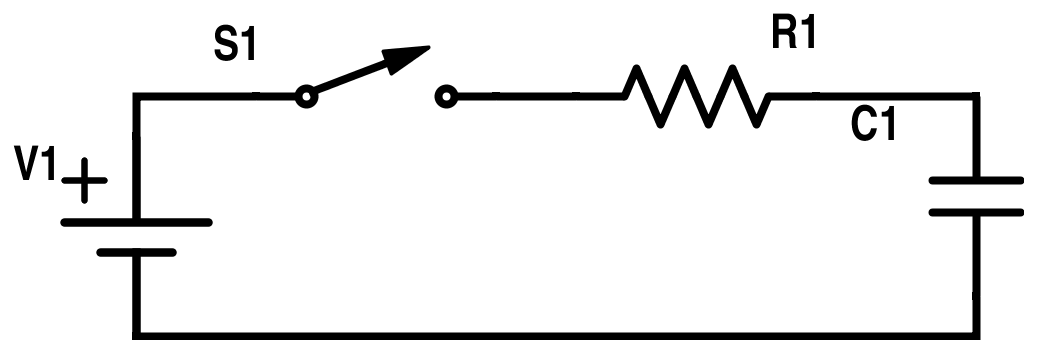
\includegraphics[width=0.8\textwidth]{assets/ece210-rc.png}
\end{center}



%%%%%%%%%%%%%%%%%%%%%%%%%%%%%%%%%%%%%%%%%%%%%%%%%%%%%%%%%%%%%%%%%%%%%%%%%%%%%%%%%%%%%%

\section*{Fourier/Transfer Function}

%%%%%%%%%%%%%%%%%%%%%%%%%%%%%%%%%%%%%%%%%%%%%%%%%%%%%%%%%%%%%%%%%%%%%%%%%%%%%%%%%%%%%%

\section*{Frequency Domain RLC}

%%%%%%%%%%%%%%%%%%%%%%%%%%%%%%%%%%%%%%%%%%%%%%%%%%%%%%%%%%%%%%%%%%%%%%%%%%%%%%%%%%%%%%

\section*{Op Amps}

%%%%%%%%%%%%%%%%%%%%%%%%%%%%%%%%%%%%%%%%%%%%%%%%%%%%%%%%%%%%%%%%%%%%%%%%%%%%%%%%%%%%%%

\section*{AM Radio/Mixing}

% SYLLABUS FROM WEBSITE
\begin{comment}
	This list comes from the ECE210 syllabus:
	Examples of signals and signal processing systems
	Analog linear time-invariant systems
	Circuits and linear systems
	Review of DC circuit analysis: KCL, KVL, dependent sources
	Capacitors and inductors as circuit elements
	Op-amp circuits
	Characterization and solution of LSI systems via linear, constant-coefficient differential equations
	Complex numbers and functions of a complex variable
	Impedance, phasors, and sinusoidal steady-state
	Frequency response and multi-frequency circuits
	Fourier Series
	Fourier transform
	AM radio
	Convolution
	Impulse and impulse response
	Sampling theorem and overview of digital signal processing
	Stability
	Laplace transform and transfer function
	Laplace transform solution of differential equations
	General form of solution to a differential equation
	Design of active filters
\end{comment}

\end{document}